\documentclass{article}

\usepackage{tikz}
\begin{document}
\pagestyle{empty}

\def\layersep{2.5cm}

% \begin{tikzpicture}[shorten >=1pt,->,draw=black!50, node distance=\layersep]
%     \tikzstyle{every pin edge}=[<-,shorten <=1pt]
%     \tikzstyle{neuron}=[circle,fill=black!25,minimum size=17pt,inner sep=0pt]
%     \tikzstyle{input neuron}=[neuron, fill=green!50];
%     \tikzstyle{output neuron}=[neuron, fill=red!50];
%     \tikzstyle{hidden neuron}=[neuron, fill=blue!50];
%     \tikzstyle{annot} = [text width=4em, text centered]

%     % Draw the input layer nodes
%     \foreach \name / \y in {1,...,4}
%     % This is the same as writing \foreach \name / \y in {1/1,2/2,3/3,4/4}
%         \node[input neuron, pin=left:Input \#\y] (I-\name) at (0,-\y) {};

%     % Draw the hidden layer nodes
%     \foreach \name / \y in {1,...,5}
%         \path[yshift=0.5cm]
%             node[hidden neuron] (H-\name) at (\layersep,-\y cm) {};

%     % Draw the output layer node
%     \node[output neuron,pin={[pin edge={->}]right:Output}, right of=H-3] (O) {};

%     % Connect every node in the input layer with every node in the
%     % hidden layer.
%     \foreach \source in {1,...,4}
%         \foreach \dest in {1,...,5}
%             \path (I-\source) edge (H-\dest);

%     % Connect every node in the hidden layer with the output layer
%     \foreach \source in {1,...,5}
%         \path (H-\source) edge (O);

%     % Annotate the layers
%     \node[annot,above of=H-1, node distance=1cm] (hl) {Hidden layer};
%     \node[annot,left of=hl] {Input layer};
%     \node[annot,right of=hl] {Output layer};
%   \end{tikzpicture}


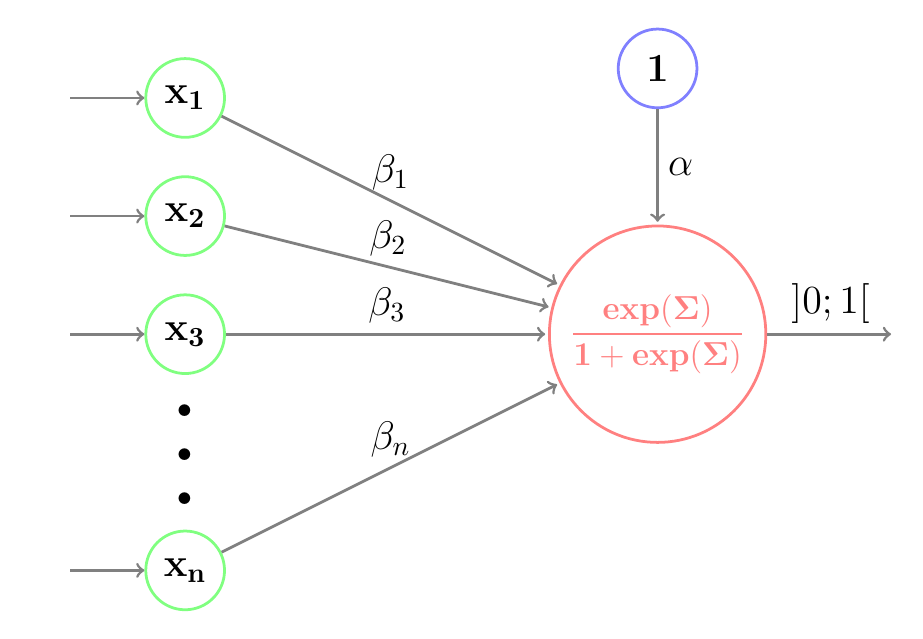
\begin{tikzpicture}[x=1.5cm, y=1.5cm, shorten >=1pt,->,draw=black!50, node distance=\layersep]
    \tikzstyle{every pin edge}=[<-,shorten <=1pt]
    \tikzstyle{neuron}=[circle,fill=black!25,minimum size=17pt,inner sep=0pt]
    \tikzstyle{input neuron}=[neuron, fill=green!50];
    \tikzstyle{output neuron}=[neuron, fill=red!50];
    \tikzstyle{hidden neuron}=[neuron, fill=blue!50];
    \tikzstyle{annot} = [text width=6em, text centered]
    \tikzset{%
    every neuron/.style={
      circle,
      line width=1pt,
    draw,
    minimum size=1cm},
    neuron missing/.style={
    draw=none, 
    scale=4,
    text height=0.333cm,
    execute at begin node=\color{black}$\vdots$},
    },
    neuron sigmastyle/.style={ 
         draw, 
         circle, 
         font=\Huge,
         minimum size=1.5cm,
         join = by -latex
       }


    \foreach \m/\1 [count=\y] in {1, 2, 3, missing, 4}
    \node [every neuron/.try, neuron \m/.try,green!50] (input-\m) at (0,2.5-\y){};% {\Large $x_\1$};

    \foreach \m [count=\y] in {1}
    \node [every neuron/.try, sigmastyle \m/.try,red!50] (output-\m) at
    (4, 2.5-3)
    {\large $\displaystyle\mathbf{\frac{exp(\Sigma)}{1+exp(\Sigma)}}$};
    %{\Huge $\displaystyle\mathbf{\Sigma}$};
    
    \foreach \m [count=\y] in {1}
    \node [every neuron/.try, neuron \m/.try,blue!50] (intercept-\m)
    at (4, 2.5-0.75){};

    \draw[](intercept-1)
    node[]{\Large $\mathbf{1}$};

    % Draw the input to the first
    \foreach \1 [count=\i] in {1, 2, 3, n}
    \draw [<-,line width=1pt](input-\i) --++(-1,0)
    node [above, midway]{}; %{\Large $\mathbf{x_\l}$};

    \foreach \1 [count=\i] in {1, 2, 3, n}
    \draw[](input-\i)
    node[]{\Large $\mathbf{x_\1}$};
    
    % Draw the input to the output
    \foreach \1 [count=\i] in {1}
    \draw [->,line width=1pt] (output-\i) --++(2,0)
    % node[above, midway]{\Large $\left]-\infty;\infty\right[$};
    node[above, midway]{\Large $\left]0;1\right[$};

    \foreach \m [count=\i] in {1, 2, 3, n}
    \foreach \j in {1}
    \draw[->, line width=1pt](input-\i) -- (output-\j)
    node[above, midway]{\Large $\beta_\m$};

    % arrow for intercept and alpha-label
    \foreach \m [count=\i] in {1}
    \foreach \j in {1}
    \draw[->, line width=1pt](intercept-\m) -- (output-\j)
    node[right, midway]{\Large $\alpha$};

\end{tikzpicture}  
% End of code
\end{document}


%%% Local Variables:
%%% mode: latex
%%% TeX-master: t
%%% End:
